\chapter{V-I Characteristics of a Diode}
	\section{Aim}
		\begin{itemize}
			\tightlist
			\item Explain the structure of a P-N junction diode
			\item Explain the function of a P-N junction diode
			\item Explain forward and reverse biased characteristics of a Silicon diode
			\item Explain forward and reverse biased characteristics of a Germanium diode
		\end{itemize}
	
	\section{Apparatus}
		\begin{itemize}
			\tightlist
			\item Silicon Diode
			\item Germanium Diode
			\item DC Battery Source
			\item Ammeter
			\item Volmeter
			\item Resistor
		\end{itemize}
	
	\section{Theory}
		\subsection{Structure of P-N junction diode}
			The diode is a device formed from a junction of n-type and p-type semiconductor material. The lead connected to the p-type material is called the anode and the lead connected to the n-type material is the cathode. In general, the cathode of a diode is marked by a solid line on the diode.
			\begin{figure}[ht]
				\centering 
				\subfloat[]{\includegraphics[width=0.45\textwidth,valign=c]{img/exp5/1}
					\label{fig:diode}}	
				\hfill
				\subfloat[]{\includegraphics[width=0.45\textwidth,valign=c]{img/exp5/2}
					\label{fig:diodeSymbol}}			
				\caption{\textit{(a) A diode (b) Symbol of a diode}}
			\end{figure}
		
		\subsection{Function of a P-N junction diode in Forward Bias}
			The positive terminal of battery is connected to the P side(anode) and the negative terminal of battery is connected to the N side(cathode) of a diode, the holes in the p-type region and the electrons in the n-type region are pushed toward the junction and start to neutralize the depletion zone, reducing its width. The positive potential applied to the p-type material repels the holes, while the negative potential applied to the n-type material repels the electrons. The change in potential between the p side and the n side decreases or switches sign. With increasing forward-bias voltage, the depletion zone eventually becomes thin enough that the zone's electric field cannot counteract charge carrier motion across the p–n junction, which as a consequence reduces electrical resistance. The electrons that cross the p–n junction into the p-type material (or holes that cross into the n-type material) will diffuse into the nearby neutral region. The amount of minority diffusion in the near-neutral zones determines the amount of current that may flow through the diode.
			
			\begin{figure}[h]
				\centering
				\includegraphics[width=0.3\linewidth]{img/exp5/3}
				\caption{Forward biased diode}
				\label{fig:pnjf}
			\end{figure}
		
		\subsection{Function of a P-N junction diode in Reverse Bias}
			The positive terminal of battery is connected to the N side(cathode) and the negative terminal of battery is connected to the P side(anode) of a diode. Therefore, very little current will flow until the diode breaks down.
			\begin{figure}[h]
				\centering
				\includegraphics[width=0.3\linewidth]{img/exp5/4}
				\caption{Reverse biased diode}
				\label{fig:pnjr}
			\end{figure}
			The positive terminal of battery is connected to the N side(cathode) and the negative terminal of battery is connected to the P side(anode) of a diode, the 'holes' in the p-type material are pulled away from the junction, leaving behind charged ions and causing the width of the depletion region to increase. Likewise, because the n-type region is connected to the positive terminal, the electrons will also be pulled away from the junction, with similar effect. This increases the voltage barrier causing a high resistance to the flow of charge carriers, thus allowing minimal electric current to cross the p–n junction. The increase in resistance of the p–n junction results in the junction behaving as an insulator.
			
			The strength of the depletion zone electric field increases as the reverse-bias voltage increases. Once the electric field intensity increases beyond a critical level, the p–n junction depletion zone breaks down and current begins to flow, usually by either the Zener or the avalanche breakdown processes. Both of these breakdown processes are non-destructive and are reversible, as long as the amount of current flowing does not reach levels that cause the semiconductor material to overheat and cause thermal damage.
		
		\subsection{Forward and reverse biased characteristics of a Silicon diode}
			\textbf{In forward biasing}, the positive terminal of battery is connected to the P side and the negative terminal of battery is connected to the N side of the diode. Diode will conduct in forward biasing because the forward biasing will decrease the depletion region width and overcome the barrier potential. In order to conduct, the forward biasing voltage should be greater than the barrier potential. During forward biasing the diode acts like a closed switch with a potential drop of nearly 0.6 V across it for a silicon diode. The forward and reverse bias characteristics of a silicon diode. From the graph, you may notice that the diode starts conducting when the forward bias voltage exceeds around 0.6 volts (for Si diode). This voltage is called cut-in voltage.
			\begin{figure}[h]
				\centering
				\includegraphics[width=1\linewidth]{img/exp5/5}
				\caption{Forward Biased Silicon diode VI plot}
				\label{fig:pnjfvi}
			\end{figure}
		
			\textbf{In reverse biasing}, the positive terminal of battery is connected to the N side and the negative terminal of battery is connected to the P side of a diode. In reverse biasing, the diode does not conduct electricity, since reverse biasing leads to an increase in the depletion region width; hence current carrier charges find it more difficult to overcome the barrier potential. The diode will act like an open switch and there is no current flow.
			
		\subsection{Forward and reverse biased characteristics of a Germanium diode}
			\textbf{In forward biasing}, the positive terminal of battery is connected to the P side and the negative terminal of battery is connected to the N side of the diode. Diode will conduct in forward biasing because the forward biasing will decrease the depletion region width and overcome the barrier potential. In order to conduct, the forward biasing voltage should be greater than the barrier potential. During forward biasing the diode acts like a closed switch with a potential drop of nearly 0.3 V across it for a germanium diode. The forward and reverse bias characteristics of a germanium diode. From the graph, you may notice that the diode starts conducting when the forward bias voltage exceeds around 0.3 volts (for Ge diode). This voltage is called cut-in voltage.
			\begin{figure}[h]
				\centering
				\includegraphics[width=1\linewidth]{img/exp5/6}
				\caption{Forward Biased Germanium diode VI plot}
				\label{fig:pnjrvi}
			\end{figure}
		
			\textbf{In reverse biasing}, the positive terminal of battery is connected to the N side and the negative terminal of battery is connected to the P side of a diode. In reverse biasing, the diode does not conduct electricity, since reverse biasing leads to an increase in the depletion region width; hence current carrier charges find it more difficult to overcome the barrier potential. The diode will act like an open switch and there is no current flow.
			
		\subsection{Diode Equation}
			In the forward-biased and reversed-biased regions, the current (\(I_f\)), and the voltage (\(V_f\)), of a semiconductor diode are related by the diode equation:
			
			$$I_f=I_s \times (exp^\frac{V_f}{n \times{V_T}}-1)$$
			
			where,
			$I_s$ is reverse saturation current or leakage current,\\
			$I_f$ is current through the diode(forward current),\\
			$V_f$ is potential difference across the diode terminals(forward voltage)\\
			$V_T$ is thermal voltage, given by
			$$V_T=\frac{k \times T}{q}$$
			
			and\\
			$k$ is \textit{Boltzmann’s constant = 1.38x10−23 J /Kelvin},\\
			$q$ is the electronic charge = \textit{1.6x10−19 joules/volt(Coulombs)},\\
			$T$ is the \textit{absolute temperature in Kelvin(K = 273 + temperature in °C)},\\
			At room temperature (25 °C), the thermal voltage is about 25.7 mV,\\
			$n$ is an \textit{empirical constant} between 0.5 and 2\\
			
			The empirical constant, $n$, is a number that can vary according to the voltage and current levels. It depends on electron drift, diffusion, and carrier recombination in the depletion region. Among the quantities affecting the value of $n$ are the diode manufacture, levels of doping and purity of materials.
			
			If n=1, the value of $\frac{k \times T}{q}$ is 26 mV at 25°C.
			When n=2, the value of $\frac{k \times T}{q}$ becomes 52 mV. For germanium diodes, n is usually considered to be close to 1. For silicon diodes, n is in the range of 1.3 to 1.6.
		
	\section{Procedure}
		\subsection{Forward Bias-Si Diode}
			\begin{enumerate}
				\tightlist
				\item Set DC voltage to 0.2 V .
				\item Select the diode.
				\item Set the resistor.
				\item Voltmeter is placed parallel to Silicon diode and ammeter series with resistor.
				\item The positive side of battery to the P side(anode) and the negative of battery to the N side(cathode) of the diode.
				\item Now vary the voltage upto 5V and note the Voltmeter and Ammeter reading for particular DC voltage.
				\begin{figure}[h]
					\centering
					\includegraphics[width=0.3\linewidth]{img/exp5/7}
					\caption{}
					\label{fig:pnjfp}
				\end{figure}
				\item Take the readings and note Voltmeter reading across Silicon diode and Ammeter reading.
				\item Plot the V-I graph and observe the change.
				\item Calculate the dynamic resistance of the diode. $R_d = \frac{\Delta V}{\Delta I}$
				\item Therefore from the graph we see that the diode starts conducting when the forward bias voltage exceeds around 0.6 volts (for Si diode). This voltage is called cut-in voltage.
			\end{enumerate}
		
		\subsection{Reverse Bias-Si Diode}
			\begin{enumerate}
				\tightlist
				\item Set DC voltage to 0.2 V .
				\item Select the diode.
				\item Set the resistor.
				\item Voltmeter is placed parallel to Silicon diode and ammeter series with resistor.
				\item The positive terminal of battery is connected to the N side(cathode) and the negative terminal of battery is connected to the P side(anode) of a diode.
				\begin{figure}[h]
					\centering
					\includegraphics[width=0.3\linewidth]{img/exp5/8}
					\caption{}
					\label{fig:pnjrp}
				\end{figure}
				\item Now vary the voltage upto 30V and note the Voltmeter and Ammeter reading for DC voltage .
				\item Take the readings and note Voltmeter reading across Silicon diode and Ammeter reading.
				\item Plot the V-I graph and observe the change.
			\end{enumerate}
		
		\subsection{Forward Bias-Ge Diode}
			\begin{enumerate}
				\tightlist
				\item Set DC voltage to 0.2 V .
				\item Use the resistor of 1K ohms and a Germanium diode.
				\item Voltmeter is placed parallel to Germanium diode and ammeter series with resistor.
				\item The positive terminal of battery is connected to the P side(anode) and the negative terminal of battery is connected to the N side(cathode) of the diode.
				\begin{figure}[h]
					\centering
					\includegraphics[width=0.3\linewidth]{img/exp5/9}
					\caption{}
					\label{fig:pnjfpge}
				\end{figure}
				\item Now vary the voltage upto 30V and note the Voltmeter and Ammeter reading for particular DC voltage .
				\item Take the readings and note Voltmeter reading across Germanium diode and Ammeter reading.
				\item Plot the V-I graph and observe the change.
				\item Therefore from the graph we see that the diode starts conducting when the forward bias voltage exceeds around 0.3 volts (for Ge diode). This voltage is called cut-in voltage.
			\end{enumerate}
		
		\subsection{Reverse Bias-Ge Diode}
			\begin{enumerate}
				\tightlist
				\item Set DC voltage to 0.2 V .
				\item Use the resistor of 1K ohms and a Germanium diode.
				\item Voltmeter is placed parallel to Germanium diode and ammeter series with resistor.
				\item The positive terminal of battery is connected to the N side(cathode) and the negative terminal of battery is connected to the P side(anode) of a diode.
				\begin{figure}[h]
					\centering
					\includegraphics[width=0.3\linewidth]{img/exp5/10}
					\caption{}
					\label{fig:pnjrpge}
				\end{figure}
				\item Now vary the voltage upto 30V and note the Voltmeter and Ammeter reading for DC voltage .
				\item Take the readings and note Voltmeter reading across Silicon diode and Ammeter reading.
				\item Plot the V-I graph and observe the change.
			\end{enumerate}

	\section{Observations}
		\begin{figure}[h!]
			\begin{longtable}[]{@{}lll@{}}
				\toprule
				Sr No. & Forward Voltage(V) & Forward Current (mA)\tabularnewline
				\midrule
				\endhead
					1 & 0.557 & 0.507\tabularnewline
					2 & 0.570 & 1.78\tabularnewline
					3 & 0.575 & 2.54\tabularnewline
					4 & 0.580 & 3.30\tabularnewline
					5 & 0.582 & 3.80\tabularnewline
					6 & 0.586 & 4.57\tabularnewline
					7 & 0.589 & 5.33\tabularnewline
					8 & 0.592 & 6.09\tabularnewline
					9 & 0.594 & 6.85\tabularnewline
					10 & 0.605 & 11.2\tabularnewline
				\bottomrule
			\end{longtable}
			\caption{Forward biased Silicon Diode}
		\end{figure}
		\begin{figure}[h!]
			\begin{longtable}[]{@{}lll@{}}
				\toprule
				Sr No. & Reverse Voltage(V) & Reverse Current (mA)\tabularnewline
				\midrule
				\endhead
				1 & 0.170 & 0.100\tabularnewline
				2 & 1.79 & 0.100\tabularnewline
				3 & 4.21 & 0.100\tabularnewline
				4 & 6.23 & 0.100\tabularnewline
				5 & 9.26 & 0.100\tabularnewline
				6 & 11.9 & 0.100\tabularnewline
				7 & 15.2 & 0.100\tabularnewline
				8 & 18.2 & 0.100\tabularnewline
				9 & 20.7 & 0.100\tabularnewline
				10 & 30.4 & 31.39\tabularnewline
				\bottomrule
			\end{longtable}
			\caption{Reverse biased Silicon Diode}
		\end{figure}
	
	
	
			
		\begin{figure}[h]
			\centering
			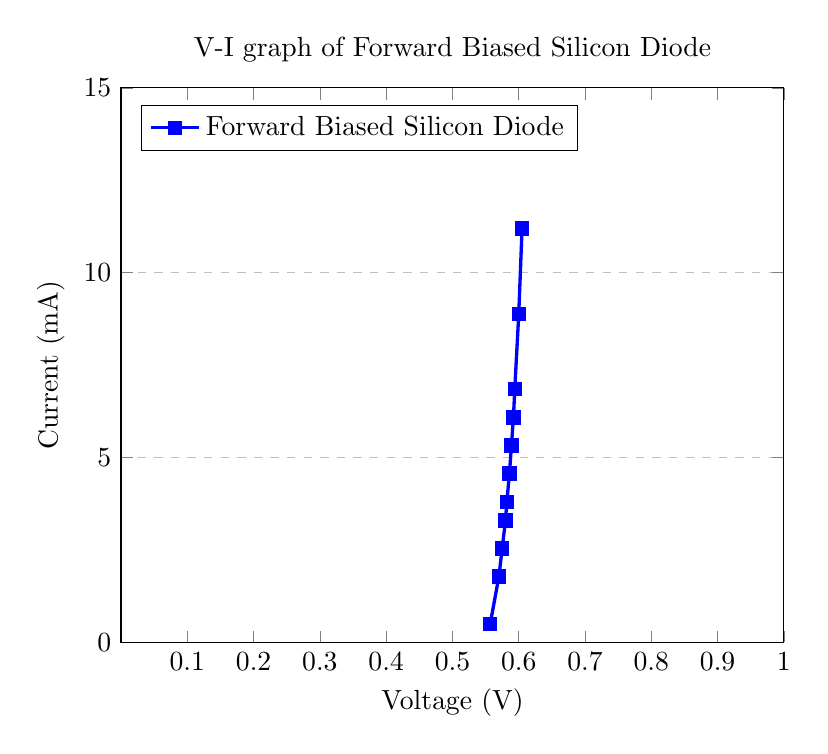
\begin{tikzpicture}
				\begin{axis}[
					title={V-I graph of Forward Biased Silicon Diode},
					width=10cm,
					xlabel={Voltage (V)},
					ylabel={Current (mA)},
					xmin=0, xmax=1,
					ymin=0, ymax=15,
					xtick={0.1,0.2,0.3,0.4,0.5,0.6,0.7,0.8,0.9,1.0},
					ytick={0,5,10,15},
					legend pos=north west,
					ymajorgrids=true,
					grid style=dashed,
					legend entries = {Forward Biased Silicon Diode}
					]
					
					\addplot[
					color=blue,
					mark=square*,
					very thick
					]
					coordinates {
						(0.557, 0.507)
						(0.570, 1.78)
						(0.575, 2.54)
						(0.580, 3.30)
						(0.582, 3.80)
						(0.586, 4.57)
						(0.589, 5.33)
						(0.592, 6.09)
						(0.594, 6.85)
						(0.600, 8.88)
						(0.605, 11.2)
					};					
				\end{axis}
			\end{tikzpicture}
			\caption{Observation $V-I$ Graph of Silicon Forward Biased Diode}
		\end{figure}
		\begin{figure}[h]
			\centering
			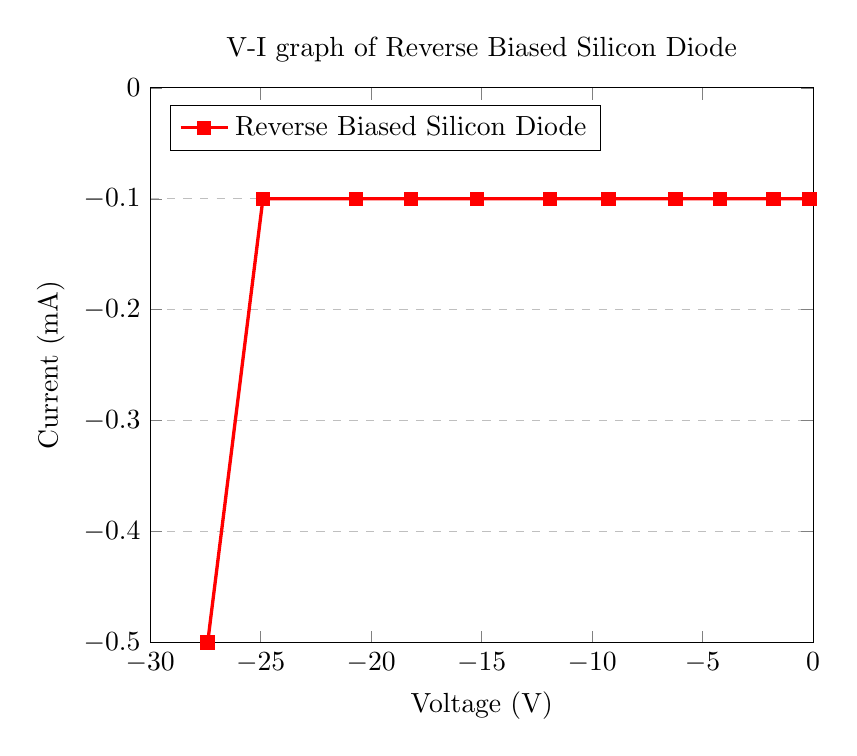
\begin{tikzpicture}
				\begin{axis}[
					title={V-I graph of Reverse Biased Silicon Diode},
					width=10cm,
					xlabel={Voltage (V)},
					ylabel={Current (mA)},
					xmin=-30, xmax=0,
					ymin=-0.5, ymax=0,
					xtick={-30,-25,-20,-15,-10,-5,0},
					ytick={-0.5,-0.4,-0.3,-0.2,-0.1,0},
					legend pos=north west,
					ymajorgrids=true,
					grid style=dashed,
					legend entries = {Reverse Biased Silicon Diode}
					]
					
					\addplot[
					color=red,
					mark=square*,
					very thick
					]
					coordinates {
						(-0.170, -0.100)
						(-1.79, -0.100)
						(-4.21, -0.100)
						(-6.23, -0.100)
						(-9.26, -0.100)
						(-11.9, -0.100)
						(-15.2, -0.100)
						(-18.2, -0.100)
						(-20.7, -0.100)
						(-24.9, -0.100)
						(-27.4, -0.5)
					};					
				\end{axis}
			\end{tikzpicture}
			\caption{Observation $V-I$ Graph of Reverse Biased Silicon Diode}
		\end{figure}
	
	\section{Result}
		A diode is a semiconductor device that essentially acts as a one-way switch for current. It allows current to flow easily in one direction, but severely restricts current from flowing in the opposite direction.
		
		When a diode allows current flow, it is forward-biased. When a diode is reverse-biased, it acts as an insulator and does not permit current to flow.
		
		